\section{Related Works}
\label{sec:related}

\noindent\textbf{Vanilla Anomaly Detection.}
Given the limited availability and high cost of abnormal images, a portion of current research on AD focuses on unsupervised methods relying exclusively on normal images~\cite{Sabokrou2018Adversarially,gong2019memorizing,US,metaformer,cutpaste,GP,ARNet,gudovskiy2022cflow,deng2022anomaly,patchcore,MKD}. Approaches such as PatchCore~\cite{patchcore} create a memory bank of normal embeddings and detect anomalies based on the distance from a test sample to the nearest normal embedding. Another method, CflowAD~\cite{gudovskiy2022cflow}, projects normal samples onto a Gaussian distribution using normalizing flows. However, relying solely on normal samples can result in an ambiguous decision boundary and reduced discriminability~\cite{bergmann2019mvtec}. In practical scenarios, a small number of anomaly samples are usually available, and these can be used to enhance detection effectiveness.

\noindent\textbf{Zero-/Few-Shot Anomaly Detection.} The utilization of a few known anomalies during training can present challenges, potentially biasing the model and hindering generalization to unseen anomalies. DRA~\cite{DRA} and BGAD~\cite{BGAD} introduce methods to mitigate this issue. Beyond simply maximizing the separation of abnormal features from normal patterns~\cite{SAD,DEVNET}, DRA~\cite{DRA} learns disentangled representations of anomalies to enable generalizable detection, accounting for unseen anomalies. BGAD~\cite{BGAD} proposes a boundary-guided semi-push-pull contrastive learning mechanism to further alleviate the bias issue. Recent advancements like WinCLIP~\cite{winclip} explore the use of foundation models for zero-/few-shot AD, leveraging language to assist in AD. Building upon WinCLIP, April-GAN~\cite{chen2023zero} maps visual features extracted from CLIP to the linear space where the text features are located, supervised by pixel-level annotated data. This paper concentrates on medical AD, a more challenging area than traditional industrial AD due to the larger gap between different data modalities.

\noindent\textbf{Medical Anomaly Detection.}
Current medical AD methods typically treat AD as a one-class classification issue, relying on normal images for training~\cite{zhou2020encoding,zhang2020viral,zhou2021proxy,zhou2021memorizing,bao2023bmad,cai2023dual,jiang2023multi}. These methods, which identify anomalies as deviations from the normal distribution, often require a large number of normal samples per class, making them impractical for real-world diagnosis. Many of these techniques are designed for a particular anatomical region~\cite{ding2022unsupervised,xu2022afsc} or are restricted to handling one specific data type per model~\cite{wolleb2022diffusion,huang2022lesionpaste,li2021unsupervised}. These methods often fall short in terms of generalizing across diverse data modalities and anatomical regions~\cite{zhang2023grace}, a pivotal aspect our paper aims to address.

\begin{figure*}[t]
    \centering    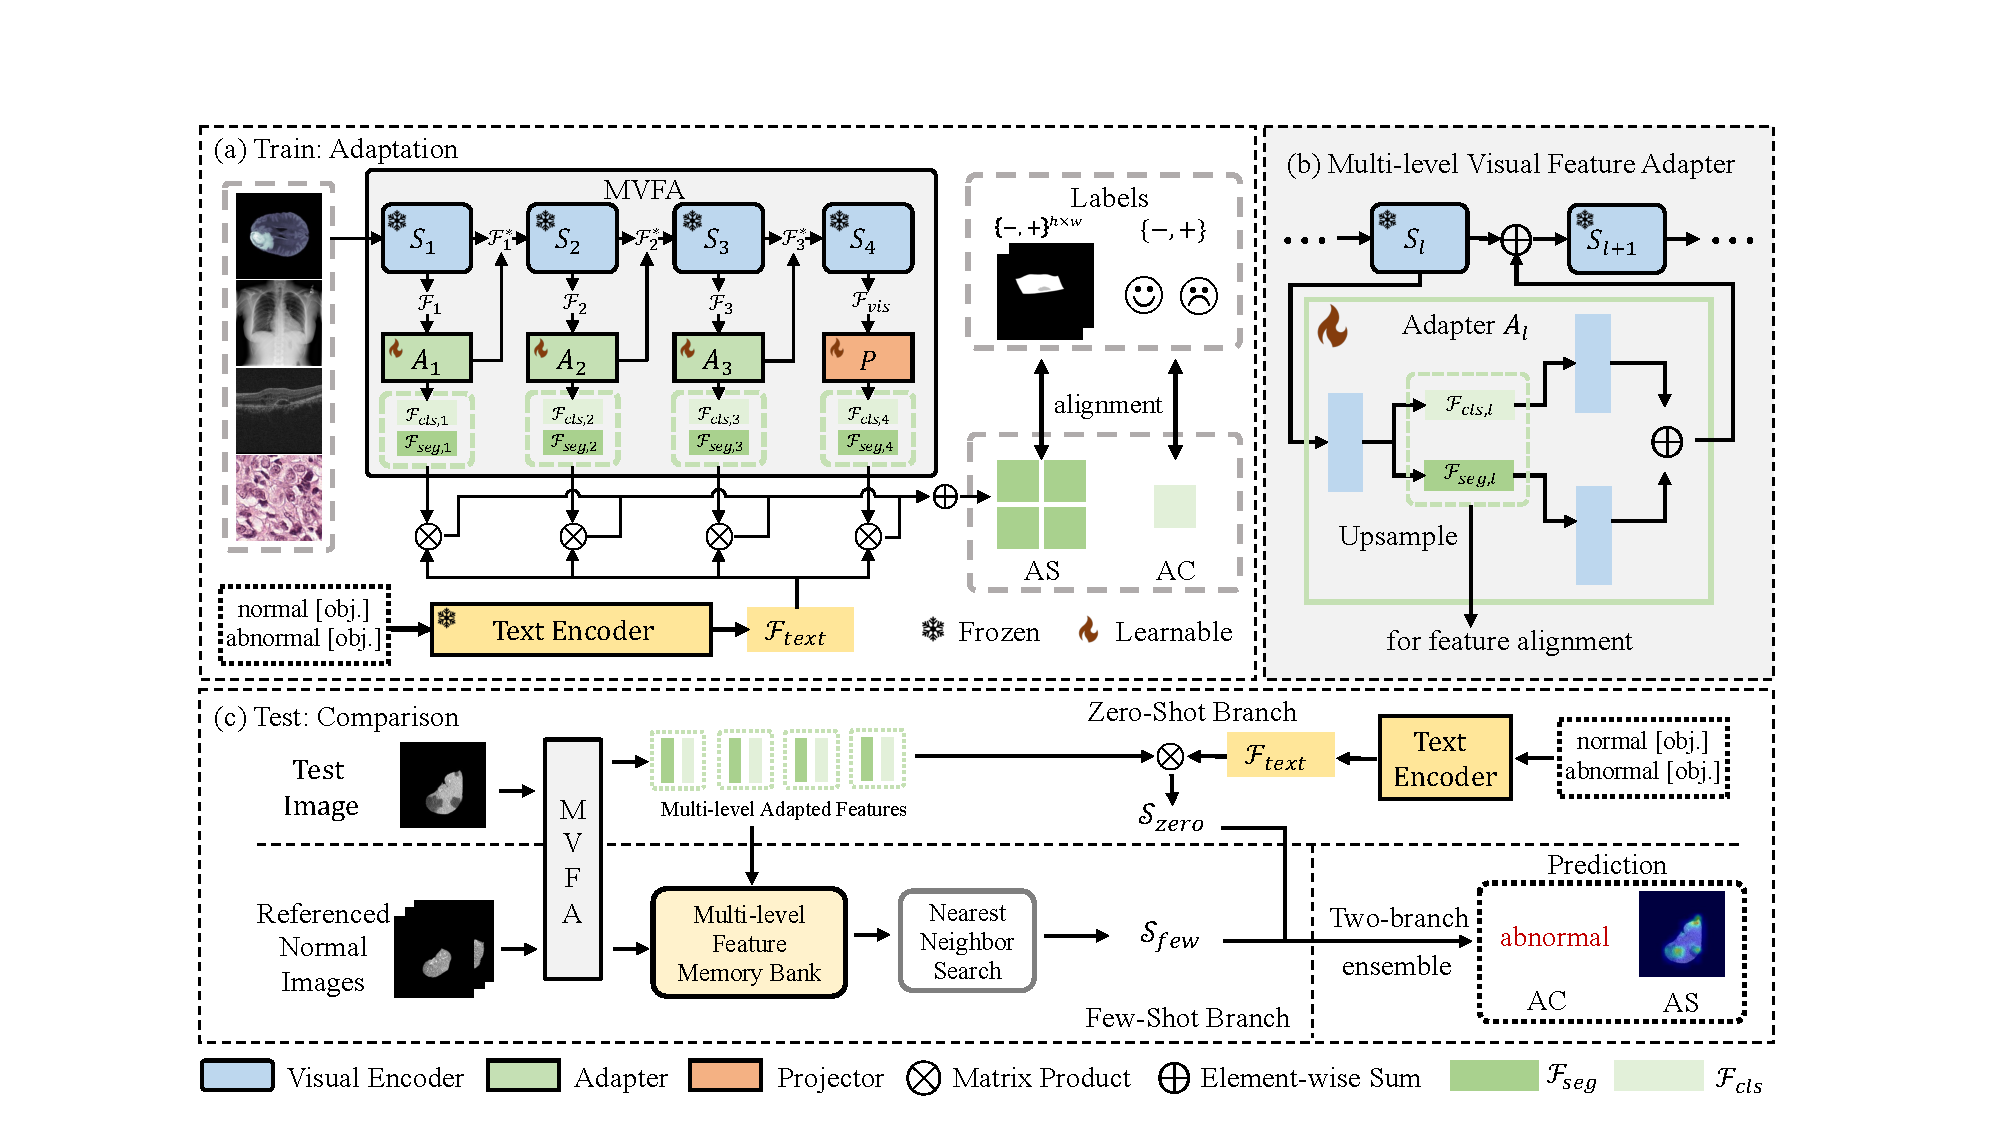
\includegraphics[width=1.0\textwidth]{img/pipeline2.pdf}
    \caption{The architecture of multi-level adaptation and comparison framework for zero-/few-shot medical anomaly detection.}
    \vspace{-7pt}
    \label{fig:pipeline}
\end{figure*}

\noindent\textbf{Visual-Language Modeling.} 
Recently, VLMs have witnessed substantial advancements, applied to many different scenarios~\cite{YuTaoCVPR23,LiXinNeurIPS23,XingyiICCV23,JingwenAAAI24,DeepCacheCVPR24,KejiNeurIPS23}. Trained on a vast amount of image-text data, CLIP~\cite{CLIP} excels in generalizability and robustness, notably enabling language-driven zero-shot inference~\cite{taori2020measuring,goh2021multimodal}. To broaden the application of VLMs, resources like the extensive LAION-5B dataset~\cite{schuhmann2022laion} and the OpenCLIP codebase~\cite{openclip} have been made available openly. Subsequent research has underscored CLIP's potential for zero-/few-shot transfer to downstream tasks beyond mere classification~\cite{gu2021open,rombach2022high,zhou2022learning}. Several studies~\cite{rao2022denseclip,zhong2022regionclip,huang2023multi} have leveraged pre-trained CLIP models for language-guided detection and segmentation, achieving promising outcomes. This research extends the application of VLMs, initially trained on natural images, to AD in medical images, introducing a unique approach of multi-level visual feature adaptation and comparison framework.